\section{Introduction}
In this chapter, we discuss our endeavour to build an ML-based system for extracting related entities from scientific text. 
Identifying named entities in the field of materials science poses a formidable challenge, particularly due to the intricate nature of material expressions, complex and extensive sequences that require meticulous attention. In this domain, the definition of materials remains elusive, lacking a clear-cut delineation (refer to Chapter~\ref{cha:introduction}). Moreover, the boundaries within materials science are loose, subject to variations based on specific subdomains, and researchers' focus on distinct aspects or phenomena associated with the materials.
Notably, within the realm of superconductor research, material expressions exhibit significant variability, incorporating various types of information within a single sequence. This can range from the chemical formula and doping ratio to the shape of the material, as exemplified by expressions such as \texttt{single crystal La x Fe 1 x O 7 (with x = 0.1, and 0.2)}. Analysing stoichiometric formulas, in particular, presents a complex task, as these necessitate resolution with substitution values scattered throughout the paper.

The complexity inherent in deciphering such material expressions has propelled our exploration into the realm of Machine Learning (ML) as a means to model these intricate boundaries. Machine learning has demonstrated its efficacy in various domains, including bioinformatics and chemistry, often surpassing rule-based or lexicon-based approaches by achieving a delicate balance between flexibility and simplicity. However, it is essential to acknowledge that the success of machine learning is contingent upon the availability of data, a facet that presents a notable challenge in materials informatics compared to other domains. This challenge, in turn, has driven us to embark on the creation of a comprehensive dataset from scratch, as detailed in Chapter~\ref{cha:supermat}.

Furthermore, the notation used in materials science may involve subscript characters, which, when converted to text, are typically normalised to a standard font size, leading to a loss of information, especially regarding subscripts. To address this, the use of Grobid has proven to be instrumental in retaining this information by leveraging PDF layout data, as expounded in Chapter~\ref{cha:pdf_extraction}. This methodological consideration enhances the precision and completeness of our named entity identification in the context of materials science.

We use various traditional machine learning (ML) methods in a unique manner within the field of materials science: linear CRF (CRF)~\cite{lafferty2001conditional}, bidirectional LSTM with CRF~\cite{lample2016neural} (BidLSTM\_CRF), bidirectional LSTM with CRF with Features~\cite{lample2016neural} (the same as (BidLSTM\_CRF) with an additional input channel for features; BidLSTM\_CRF\_FEATURES), and fine-tuned SciBERT-based~\cite{Beltagy2019SciBERT} encoder using a CRF as the activation layer (Scibert).
Our contribution lies in the innovative use of the cascade approach for material recognition, which differs from previous research focussing mainly on extracting formulas. Although existing work, such as \cite{kononova2019text, court2020magnetic, dieb2015framework}, concentrates on formula extraction, our objective is to extract as large a sequence as possible and subsequently address material segmentation separately. This methodology enables the reusability of components, such as the material parser, in different contexts and domains.

Our approach also uses positive sampling as a novel method to boost the recall, which, interestingly, results in better results overall as compared with the traditional approximation.

Chapter~\ref{cha:supermat} presents a comprehensive description of the data model, including the data type and their example, which have been considered by domain experts for constructing the training and evaluation dataset: SuperMat. 


\section{Proposed solution}

This process is organised into two stages: initially, we apply Named Entity Recognition (NER) on the content extracted in the previous steps to identify and extract significant entities.
Next, we ran a relation extraction (RE) task was conducted on the identified entities and the context in which they were appearing.

The approach for NER involves prioritizing recall over precision. In other words, the goal is to capture as many entities as possible, even if it means sacrificing precision scores. This means that while some unrelated entities may be extracted, they are likely to be filtered out in the subsequent step of relation extraction.
However, we adjusted the RE to be more cautious, favoring higher precision. This is because the final outcome is expected to undergo human validation. If the RE has a high recall, it may affect its efficiency as the validator would have to spend a significant amount of time removing numerous incorrect records.
From a holistic perspective, the recall-precision bias will be balanced between the two processes, as evidenced by the end-to-end evaluation results, which will be further discussed in Section~\ref{sec:end2end}.

ML models are interfaced by Grobid, which uses the Wapiti\cite{lavergne2010practical} implementation for linear CRF, and DeLFT (Deep Learning for Text)~\cite{DeLFT} for deep learning models.
The architectures CRF and BidLSTM\_CRF\_FEATURES make use of the orthogonal features that we have summarised in Table~\ref{tab:ML-model-features}.

\begin{sidewaystable}[ht]
    \centering
    \caption{Summary of the features used in the \textit{superconductors} and \textit{material} ML models. \textit{All} under Architecture indicate only BidLSTM\_CRF\_FEATURES and CRF.}
    \begin{tabular}{l m{30em} c c}
        \toprule
        \textbf{\#}   & \textbf{Feature}                                                                                                                                                                                                                                         & \textbf{Model}  & \textbf{Architecture} \\
        \midrule
        \textbf{1}    & current token                                                                                                                                                                                                                                            & all             & all                   \\
        \textbf{2}    & current token lower cased                                                                                                                                                                                                                                & all             & all                   \\
        \textbf{3-6}  & (four features) current token, prefix characters 1 to 4                                                                                                                                                                                                  & all             & CRF                   \\
        \textbf{7-10} & (four features) current token, suffix characters 1 to 4                                                                                                                                                                                                  & all             & CRF                   \\
        \textbf{11}   & information about capitalisation: first character (INITCAP), all characters (ALLCAPS), none (NOCAPS)                                                                                                                                                     & all             & all                   \\
        \textbf{12}   & digits content: all (ALLDIGIT), some digits (CONTAINDIGIT), no digits (NODIGIT)                                                                                                                                                                          & all             & all                   \\
        \textbf{13}   & (boolean) the token is composed by a single character                                                                                                                                                                                                    & all             & all                   \\
        \textbf{14}   & punctuation information and normalisation to placeholders: no punctuation (NOPUNCT), open or end brackets (OPENBRACKET, ENDBRACKET), various punctuation (DOT, COMMA, HYPHEN, QUOTE), open or close quotes (OPENQUOTE, ENDQUOTE), anything else (PUNCT) & all             & all                   \\
        \textbf{15}   & Shadow the numbers                                                                                                                                                                                                                                       & all             & CRF                   \\
        \textbf{16}   & Shadow any characters: ``x'' for lowercase, ``X'' for uppercase, ``d'' for digits                                                                                                                                                                        & all             & CRF                   \\
        \textbf{17}   & As the previous but compressed                                                                                                                                                                                                                           & all             & CRF                   \\
        \textbf{18}   & Font name                                                                                                                                                                                                                                                & superconductors & all                   \\
        \textbf{19}   & Font size                                                                                                                                                                                                                                                & superconductors & all                   \\
        \textbf{20}   & Font style: standard (BASELINE), superscript (SUPERSCRIPT) or subscript (SUBSCRIPT)   & superconductors & all                   \\
        \textbf{21}   & (boolean) if the token style is bold & superconductors & all                   \\
        \textbf{22}   & (boolean) if the token style is italic & superconductors & all                   \\
        \textbf{23}   & (boolean) the token is identified as a chemical compound by ChemDataExtractor\cite{chemdataextractor}                                                                                                                                                    & superconductors & all                   \\
        \bottomrule
    \end{tabular}
    \label{tab:ML-model-features}
\end{sidewaystable}

\subsection{NER}
\label{subsec:ner-solution}

The implementation of NER follows the cascade approach (Figure~\ref{fig:extraction-ml-models-cascade-architecture}), where models are applied in cascade from a broader to a more specific scope. This approach requires models to be specialised in single or simple tasks, which makes their construction simpler and requires less complex data. 
In fact, this method allows us to simplify the end-to-end task to smaller subtasks where specific models may be reused in different parts of the process when they require performing the same task. 

\begin{figure}[htbp]
    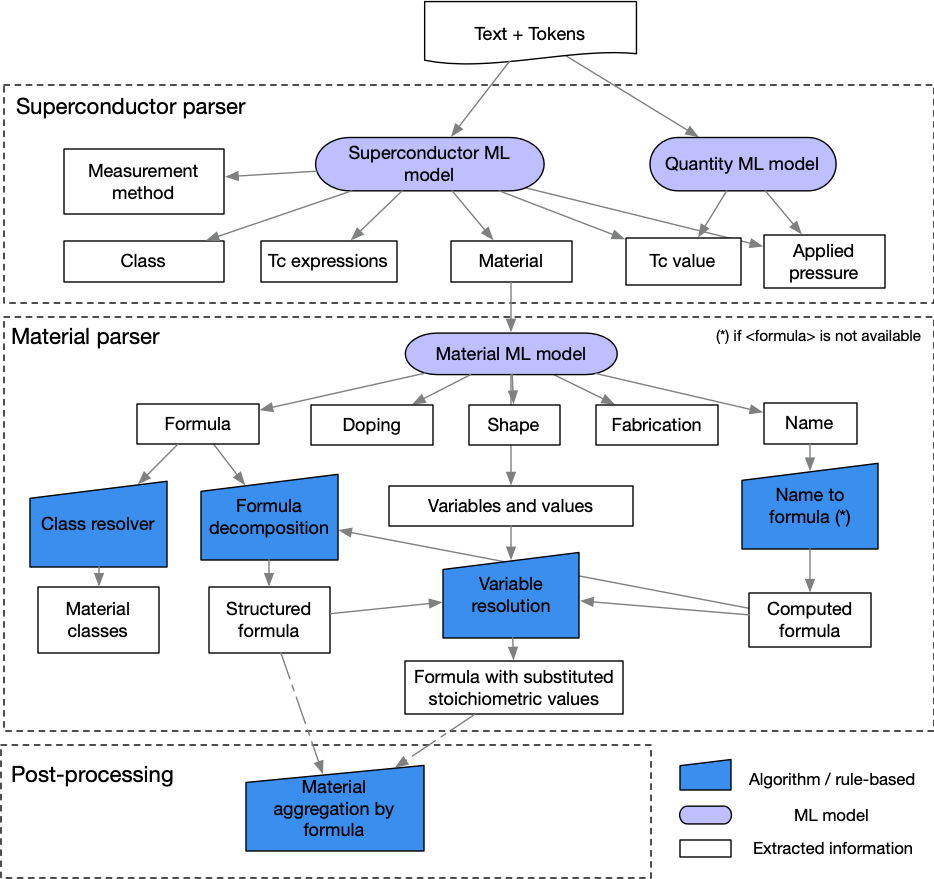
\includegraphics[width=\textwidth]{figures/automatic_extraction_supercon/schema-extraction-colors}
    \caption{\label{fig:extraction-ml-models-cascade-architecture} Cascade architecture in the NER step. The white rectangles indicate the extracted information (described in Tables~\ref{tab:superconductors-parser-entities} and~\ref{tab:material-parser-entities}).}
\end{figure}

The schema illustrated in Figure~\ref{fig:extraction-ml-models-cascade-architecture} is made up of three main components: the ``superconductor parser'', the ``material parser'' and the ``post-processing''. 

\subsubsection{Superconductor parser}
The ``superconductor parser'' extracts first-level entities (Table~\ref{tab:superconductors-parser-entities} by aggregating the resulting entities from two ML models: ``Superconductors ML model'' and ``Quantities ML model''.
The ``Quantities ML model'' is reused from a separate Grobid module for the measurement and extraction of physical quantities~\ref{cha:measurements} and is limited in scope to only target entities of temperatures and pressures.
Overlapping entities of temperatures and pressures are merged, exact duplicates are removed, and the largest entities (in terms of string length) are preserved.
The ``Superconductors ML model'' was trained with SuperMat (Chapter~\ref{cha:supermat}), whose schema is summarised in Table~\ref{tab:superconductors-parser-entities}.
As discussed above, we boosted the recall for the NER task as a novel characteristic compared to other methods.
We trained the model by applying positive sampling, which consists of removing examples that do not contain any entities (negative examples, Figure~\ref{fig:training-holdout-set-distribution}a).
This approach provided an improvement of 2\% in both precision and recall compared to the result without sampling.
We tested additional sampling approaches, called active and random sampling, that target highly imbalanced datasets~\cite{lopez2021mining}. We tested them using ratios of negative examples of 0.1, 0.25, 0.5 and 1.0, however, they did not provide stable evidence suggesting any improvement as compared with our positive sampling approach. 

\begin{table}[ht]
    \centering\small
    \caption{Entities extracted by the superconductors parser.}
    \begin{tabular}{m{10em} m{20em}}
        \toprule
        \textbf{Entity} (\textbf{tag})              & \textbf{Description} \\
        \midrule
        Material (\texttt{<material>})              & Materials and samples names, formulas (including stochiometric formulas), substitution variables of values and elements, shape, doping, and substrate               \\
        Class (\texttt{<class>})                    & Groups of materials having similar characteristics or common strategic compounds that define their nature                                                      \\
        \tc value (\texttt{<tcValue>})      & The value of the superconductor critical temperature                                                                                                          \\
        \tc expressions (\texttt{<tc>})     & Expressions in the text that provide information about the phenomenon of superconductivity related to a value, interval or variation of \tc \\
        Measurement method (\texttt{<me\_method>}) & Technique used to measure or calculate the presence of superconductivity                                                                                     \\
        Applied pressure (\texttt{<pressure>})      & Applied pressure when superconductivity is recorded                                                                                                            \\
        \bottomrule
    \end{tabular}
    \label{tab:superconductors-parser-entities}
\end{table}

Entities of type \texttt{<material>}, which may contain heterogeneous mixed information, are passed in the cascade to the ``Material parser'', which aggregates ML and rule-based methods.

\subsubsection{Material Parser}

The Material Parser is an expression of different approaches. 
First, the entity is passed through a novel Material ML model to segment and identify its content (Table~\ref{tab:material-parser-entities}).
Then, different processes are applied depending on which information is available: 
\begin{itemize}
    \item Formulas are decomposed into a structured composition. We identify each element-stoichiometry pair (e.g., ``O'': 7.0) using mat2chem~\cite{kononova2019text} and Pymatgen~\cite{Ong2013}; if only the material name is available, we lookup its formula (e.g., hydrogen to \textit{H}),
    \item Using heuristics, we classify the formula by assigning multiple classes as they are understood from superconductor researchers, for example cuprate, oxides, alloys, etc.
    \item Using the variables and values extracted, we substitute them into partial formulas. For example, in \texttt{La 4 Fe 2 A 1-x O 7 (A=Mg,Co; x=0.1,0.2)}, we substitute \textit{A} and \textit{x} using their parsed values, and applying permutations, we obtain four \textit{resolved formulas}: \texttt{La 4 Fe 2 Mg 0.9 O 7}, \texttt{La 4 Fe 2 Mg 0.8 O 7}, \texttt{La 4 Fe 2 Co 0.9 O 7}, and \texttt{La 4 Fe 2 Co 0.8 O 7}.
\end{itemize}

\begin{table}[ht]
    \centering\small
    \caption{Entities extracted by the material parser. }

    \begin{tabular}{m{10em} m{20em}}
        \toprule
        \textbf{Entity} (\textbf{tag})               & \textbf{Description}                                                                                                              \\
        \midrule
        Name (\texttt{<name>})                       & The canonical name of a material (e.g., hydrogen, PCCO, carbon)                                                                    \\
        Formula (\texttt{<formula>})                 & Chemical formula of the material (e.g., \texttt{Pr1.869Ce0.131CuO 4-}, \texttt{MgB2}, \texttt{La 2-x Sr x CuO 4})                  \\
        Doping (\texttt{<doping>})                   & Doping ratio and doping materials that are adjoined to the material name (e.g., \texttt{Zn-doped}, \texttt{2\% Zn-doped})          \\
        Shape (\texttt{<shape>})                     & shape of the material (e.g. single crystal, polycrystalline, thin film, powder, film)                                             \\
        Substitution variables (\texttt{<variable>}) & Variables that can be substituted in the formula.                                                                                 \\
        Substitution values (\texttt{<value>})       & Values expressed in the doping.                                                                                                   \\
        Substrate (\texttt{<substrate>})             & Substrates as defined in the material name                                                                                        \\
        Fabrication (\texttt{<fabrication>})         & Additional information that does not belong to any of the previous tags  (e.g., intercalated, electron-doped) \\
        \bottomrule
    \end{tabular}
    
    \label{tab:material-parser-entities}
\end{table}


\subsubsection{Post-processing}
Finally, after all entities are extracted, the post-processing aggregates different mentions of the same materials using the parsed formulas at the document-level.
For example, formula with partial substitutions such as \texttt{La 2 Fe 1-x O 7 (x = 0.1, 0.2)} will be aggregated with materials like \texttt{La 2 Fe 0.9 O 7} appearing in other sections of the same document.


\subsection{RE}
\label{subsec:re-solution}
\label{subsubsec:linking}

Relation extraction (RE) links materials and their corresponding properties. 
We explored different approaches, such as the use of dependency parsing~\cite{yoshikawa:2017acl, Tiktinsky2020pyBARTES, swayamdipta:17, zhou-zhao-2019-head} or machine learning~\cite{lin2016neural,hariharan2019relation}. 
These methods were developed or trained using text from news articles, and their performances on scientific text were not satisfactory. 
Another aspect is that our dataset was too small to successfully train any of these ML methods. 
In particular, working with dependency parsers was extremely difficult, due to their inability to districate in such complex writing. 
Compensating such poor performances resulted in the need to write over-complicated rules. 


In our algorithm, pairs of entities are linked focusing on three types of link:
\begin{itemize}
    \item \textbf{material-tcValue}: The link between a material and its corresponding \tc.
    \item \textbf{tcValue-pressure}: The link between \tc and its related critical pressure.
    \item \textbf{me\_method-tcValue}: The link between \tc and its corresponding measurement method.
          % \item \textbf{material-crystal\_structure} link the material with their crystal structure, and 
          % \item \textbf{material-space\_group} to link the material to their space groups.
\end{itemize}

Entities of type \texttt{<tcValue>} are pre-processed through a classifier that establishes whether or not they temperatures related to the superconductivity. This is used to exclude other temperatures (e.g., annealing, transition, Curie) that might be incorrectly extracted by the previous step.
This rule-based classifier combines the extracted entities of \tc expressions (label \texttt{<tc>}) with a set of predefined standard terms.
If a temperature is not considered a \tc, it is excluded from the list of possible linking candidates.

Two scenarios are considered. First, if entities to be linked in the sentence are only two they are linked automatically, else further rules are applied. 
If the word ``respectively'' appears in the sentence, we apply ``order-linking''. 
For example, consider the following sentence:
\begin{displayquote}
    P-or Ba-122  and Co-doped Ba-122 have lower \tc's of about 30 K and 24 K, respectively, which makes helium free operation questionable.
\end{displayquote}
It contains the word ``respectively'', and by applying ``order-linking'', \textit{P-or Ba122} is assigned to \textit{30 K} and \textit{Co-doped Ba-122} to \textit{24 K}.


If the word ``respectively'' does not appear in the sentence, we apply ``distance linking'' which works by defining the distance measurement \textit{d} as a value calculated as the number of characters between the centroid of each entity.
Entities surrounded by parentheses are expanded to the whole parentheses, and its centroid is updated.
As an example, in the sentence
\begin{displayquote}
    We tested two materials MgB2 (Tc = 39 K) and FeSe (Tc = 16 K).
\end{displayquote}

\texttt{39 K} is closer to \texttt{FeSe} (\textit{d}=10) than to \texttt{MgB2} (\textit{d}=11). 
In this example, however, both temperatures entities would be expanded to their containing parenthesis (e.g. ``\texttt{39 K}'' to ``\texttt{(Tc = 39 K)}''. 
In this case, the centre of the entity ``\texttt{39 K}'' is shifted to the left, from the initial value of 38 to 35 and the distance from \texttt{MgB2} is reduced from \textit{d}=11 to \textit{d}=8.
As a result, the \texttt{MgB2} entity is correctly linked to ``\texttt{39 K}''.

Distance calculation is also adjusted with the addition of ``penalties'' by doubling the calculated distance when certain keywords or punctuations (``,'', ``.'', ``;'', ``and'', ``but', ``while', ``whereas', ``which'', ``although'') appear between two entities because they represent a logical separation of predicates ~\cite{oka2021table}.
In the above example, the distance between \texttt{39 K} and \texttt{FeSe} would be doubled (\textit{d}=20) and the link would not be made.

\section{Results}

\subsection{Superconductor ML model NER Evaluation}
\subsubsection{Experimental settings}

We used SuperMat~\ref{cha:supermat} for training (76\% (132 documents)) and evaluation (24\%, 32 documents). 

The holdout set evaluation consists of using a fixed part of a dataset for validation. 
Selection must be performed to reproduce the same distribution of entities from the original dataset.
We assembled the holdout set by manually selecting 32 documents (24\%) from SuperMat, making sure they had a similar ratio of examples, entities and unique entities with the remaining 76\% (132 documents) which was used as training set (Figure~\ref{fig:training-holdout-set-distribution}a).
Maintaining the same rate for the distribution of entities types between the two sets was more challenging: on average, we obtained approximately 15 18\% labels of each type in the holdout set (Figure~\ref{fig:training-holdout-set-distribution}b), except for the \texttt{<material>} label (23\%). 

\begin{figure}[ht]
    \centering
    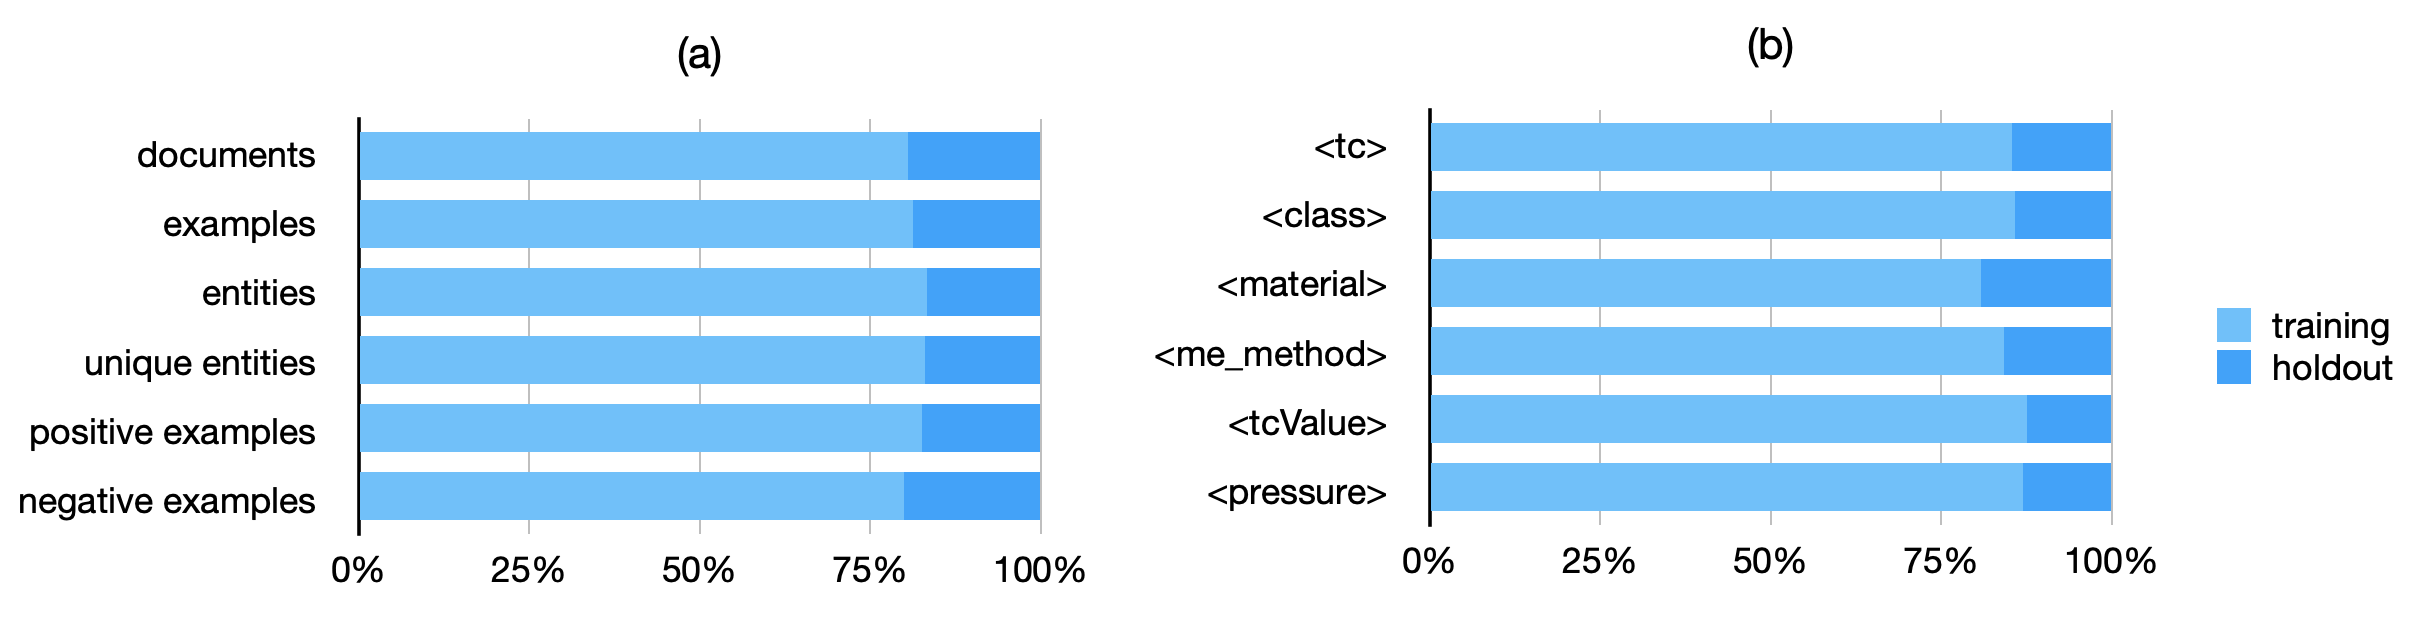
\includegraphics[width=\textwidth]{figures/automatic_extraction_supercon/superconductor-holdout-training-set}
    \caption{Holdout/training set distribution for (a) general metrics and (b) entity labels; entities and unique entities indicate the number of labelled entities with and without value duplicates, respectively, and positive examples (+) and negative examples (-) indicate the number of sentences with at least one entity and with no entities, respectively.}
    \label{fig:training-holdout-set-distribution}
\end{figure}

\begin{figure}[ht]
    \centering
    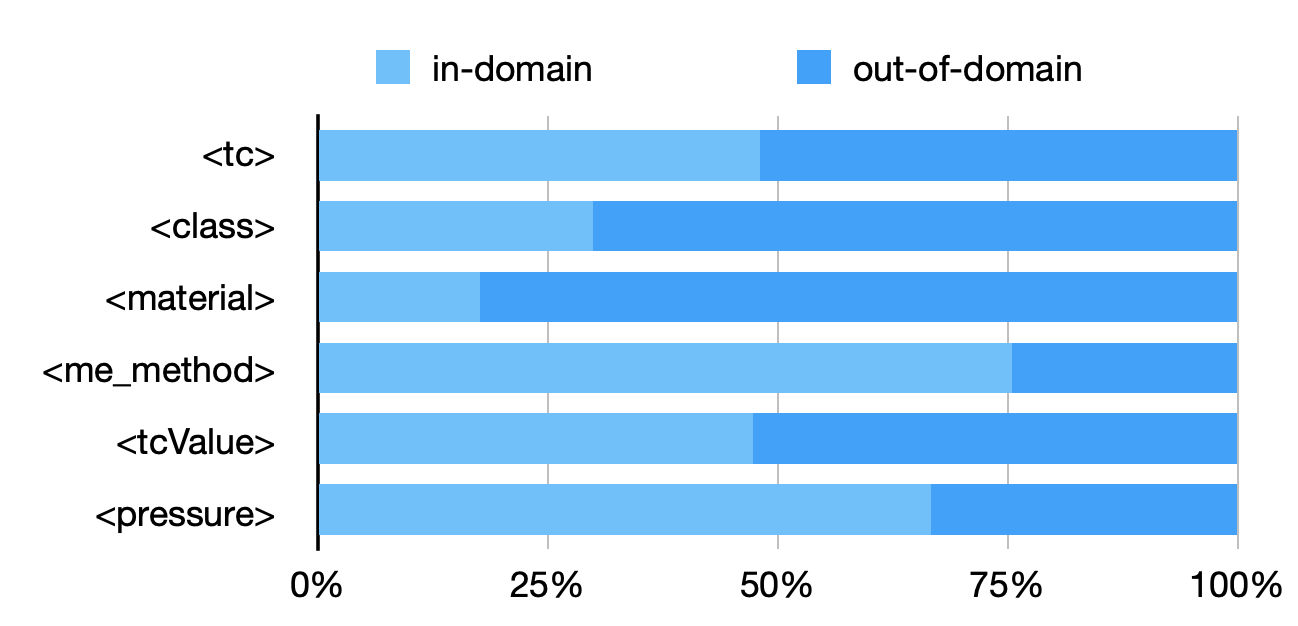
\includegraphics[width=0.6\textwidth]{figures/automatic_extraction_supercon/superconductor-out-domain-holdout-unique}
    \caption{Holdout ``out-of-domain'' rates. The entities from the holdout set that are also in the training set are ``in-domain'' and the entities that are not in the training set are ``out-of-domain''.}
    \label{fig:out-domain-holdout}
\end{figure}

We defined the ``out-of-domain'' ratio as the number of unique entities from the holdout set that were not in the training set.
The holdout set ``out-of-domain'' ratio was on average around 72\%, which challenges the model generalisation (every 100 entities in the holdout set, 72 were never seen before during training).
Most labels had an ``out-of-domain'' ratio above 50\%  (Figure~\ref{fig:out-domain-holdout});  \texttt{<material>}, the most important label, had the highest ratio (82\%) while \texttt{<me\_method>} and \texttt{<pressure>} have the lowest (25\% and 33\%). 
The low ratio of \texttt{<me\_method>} can be explained by their low entity variability (11.44\%).

\subsubsection{Results}
We performed the evaluation by repeating the training and evaluation 5 times: while the training and evaluation dataset are fixed, the way the dataset are provided to the model is randomly shuffled at each run, adding some entropy in the training, which is visible as a variability in the evaluation scores.
The results are then averaged as reported in Table~\ref{tab:evaluation-superconductors-ML-model}.

Scibert obtained the best results with an F1 of 77.03\% and a recall of around 80.69\% (Table~\ref{tab:evaluation-superconductors-ML-model}).
The features did not provide any improvements with RNN models: BidLSTM\_CRF and BidLSTM\_CRF\_FEATURES resulted in the same F1 score.
This result comes as a surprise because features such as superscript/subscript were expected to be determinants for recognising material sequences.


\begin{sidewaystable}[htbp]
    \centering\small
    \caption{Evaluation scores (\%) for the Superconductor ML model in the four architectures. For the DL architecture, the results are averaged over 5 runs. Support (Supp) indicates the number of labels in the training data. Values in bold indicate the highest score. P: precision, R: recall.}
    
    \scalebox{0.8}{
        \begin{tabular}{l ccc ccc ccc ccc r}
            \toprule
            \textbf{Label}        & \multicolumn{3}{c}{\textbf{CRF}} & \multicolumn{3}{c}{\textbf{BidLSTM\_CRF}} & \multicolumn{3}{c}{\makecell{\textbf{BidLSTM\_CRF}                                                                                                                                                 \\\textbf{\_FEATURES}}} & \multicolumn{3}{c}{\textbf{Scibert}} & \textbf{Supp} \\
            \cmidrule(lr){2-4}\cmidrule(lr){5-7}\cmidrule(lr){8-10}\cmidrule(lr){11-13}\cmidrule(lr){14-14}
                                  & \textbf{P}                       & \textbf{R}                                & \textbf{F1}                                        & \textbf{P} & \textbf{R} & \textbf{F1}    & \textbf{P}     & \textbf{R} & \textbf{F1}    & \textbf{P} & \textbf{R}     & \textbf{F1}    &      \\
            \midrule
            \texttt{<class>}      & 79.74                            & 66.79                                     & 72.69                                              & 79.01      & 72.62      & \textbf{75.66} & 77.84          & 72.40      & 74.97          & 72.95      & 75.28          & 74.09          & 1646 \\
            \texttt{<material>}   & 79                               & 72.15                                     & 75.42                                              & 79.25      & 76.94      & 78.06          & 81.07          & 75.10      & 77.94          & 80.15      & 81.42          & \textbf{80.77} & 6943 \\
            \texttt{<me\_method>} & 60.25                            & 68.73                                     & 64.21                                              & 56.41      & 79.49      & 65.92          & 55.86          & 80.45      & 65.90          & 56.26      & 81.52          & \textbf{66.56} & 1883 \\
            \texttt{<pressure>}   & 46.15                            & 29.27                                     & 35.82                                              & 49.45      & 58.05      & 52.53          & 50.25          & 60.49      & \textbf{54.36} & 41.72      & 52.68          & 46.51          & 274  \\
            \texttt{<tc>}         & 84.36                            & 83.57                                     & \textbf{83.96}                                     & 78.61      & 82.54      & 80.48          & 79.19          & 82.07      & 80.60          & 74.46      & 82.66          & 78.35          & 3741 \\
            \texttt{<tcValue>}    & 69.8                             & 66.24                                     & 67.97                                              & 70.36      & 75.16      & 72.67          & 68.95          & 76.56      & 72.52          & 70.90      & 79.74          & \textbf{75.06} & 1099 \\
            \midrule
            All (micro avg)       & 76.88                            & 72.77                                     & 74.77                                              & 74.59      & 77.67      & 76.09          & \textbf{75.17} & 76.79      & 75.96          & 73.69      & \textbf{80.69} & \textbf{77.03}        \\
            \bottomrule
        \end{tabular}
    }
    
    \label{tab:evaluation-superconductors-ML-model} 
\end{sidewaystable}

The \texttt{<pressure>} label had the lowest performance scores in all architectures. We believe that 274 training examples are not a sufficient large number considering that pressure expressions can be dependent on the context because they can refer to different types of pressures (e.g., annealing pressure).
The label with the highest score was \texttt{<material>}, with F1 values of 80.77\% and 78.06\% for Scibert and BidLSTM\_CRF, respectively. In addition, \texttt{<material>} had the highest ``out-of-domain'' ratio in the holdout set (greater than 75\%, Figure~\ref{fig:out-domain-holdout}) and the highest ``label variability'' (the ratio between unique entities and total entities, about 42\%), which suggests that the model recognises correctly materials that has not been ``seen'' during the training.
On the other hand, the \texttt{<me\_method>} label, which has lower ``label variability'' (around 11\%) and a low ``out-of-domain'' ratio, had an F1 score of 66.56\% with Scibert and 65.92\% with BidLSTM\_CRF.
For \texttt{<tc>}, the CRF outperformed the other architectures (F1 score of 83.96\%), especially Scibert (78.35\%). 
This outcome can be explained by the extremely low variability (12.69\%) of entities labelled as \texttt{<tc>}. %, and having the holdout set with a balanced average ``out-of-domain'' ratio 51\%. 
% The entity labels variability (ratio of unique entities versus the total) is, in average, around 55\%, and 57\% for the training and holdout sets, respectively. \texttt{<tc>} (12\%) and \texttt{me\_method} have the lowest variability while the \texttt{<material>} has the highest. 

\begin{figure}[htbp]
    \centering
    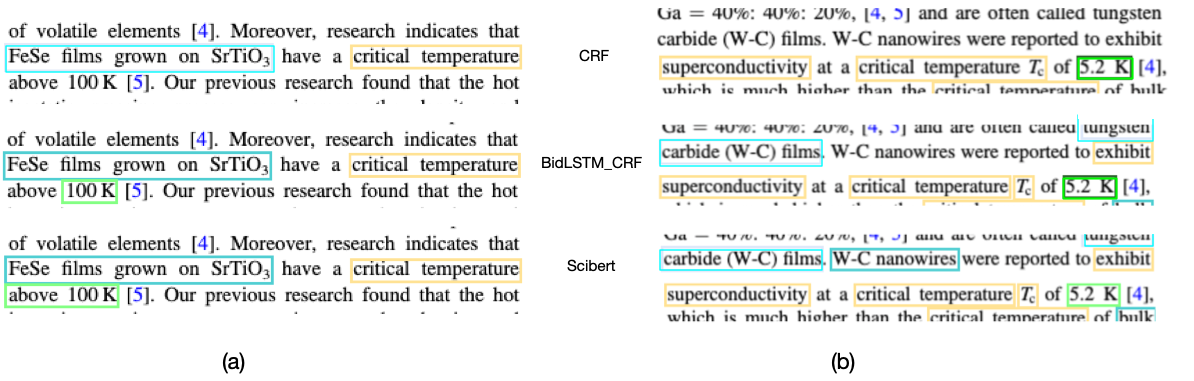
\includegraphics[width=\textwidth]{figures/automatic_extraction_supercon/example-comparison-archs.png}
    \caption{Examples taken from two sources~\cite{Gajda_2016, Shibata_2016} of results from three different architectures: CRF, BidLSTM\_CRF and, Scibert. The boxes annotating the text represent the extracted entities (material are indicated in light blue, \tc in green, and \tc expressions in yellow).}
    \label{fig:example-comparison-architectures}
\end{figure}

Scibert shows good generalisation capacity for unseen examples or examples appearing in different contexts.
For example, in Figure~\ref{fig:example-comparison-architectures}a, only Scibert correctly extracts ``above 100K'', while CRF misses it completely and BidLSTM\_CRF misses ``above''.
In the training data, ``above 100K'' is not present, but ``below 100K'' and ``\~100K'' are present, and several other entities contain the token ``above'' and Scibert can understand that the token ``above'' is relevant to the temperature.
In a second example (Figure~\ref{fig:example-comparison-architectures}b), only Scibert can correctly extract ``W-C nanowire'' which is not present in the SuperMat training data.
Unfortunately, we cannot check whether ``above 100K'' or ``W-C nanowire'' are also present in the dataset used in the pre-train of SciBERT by their authors~\cite{Beltagy2019SciBERT} because the data are not available.


\subsection{Material parser segmentation model}

We trained the Material ML model using SuperMat, we created a new layer of annotations generated for each entity of type \texttt{<material>} in the top layer set of annotations of SuperMat. The resulting entities illustrated in Table~\ref{tab:material-parser-entities} include the different information included in the material entities.
We trained the same architecture as for the ``Superconductors ML model''.

\subsubsection{Experimental settings}

In this model, we created an independent holdout set because manual annotation is performed on smaller chunks of text and requires less effort than annotating sentences as when we developed SuperMat.
We used material data extracted from a dataset of 500 documents (500-papers) from three publishers: \textit{American Institute of Physics} (AIP), \textit{American Physical Society} (APS) and \textit{Institute of Physics} (IOP)~\cite{foppiano2019proposal}.

\begin{figure}[ht]
    \centering
    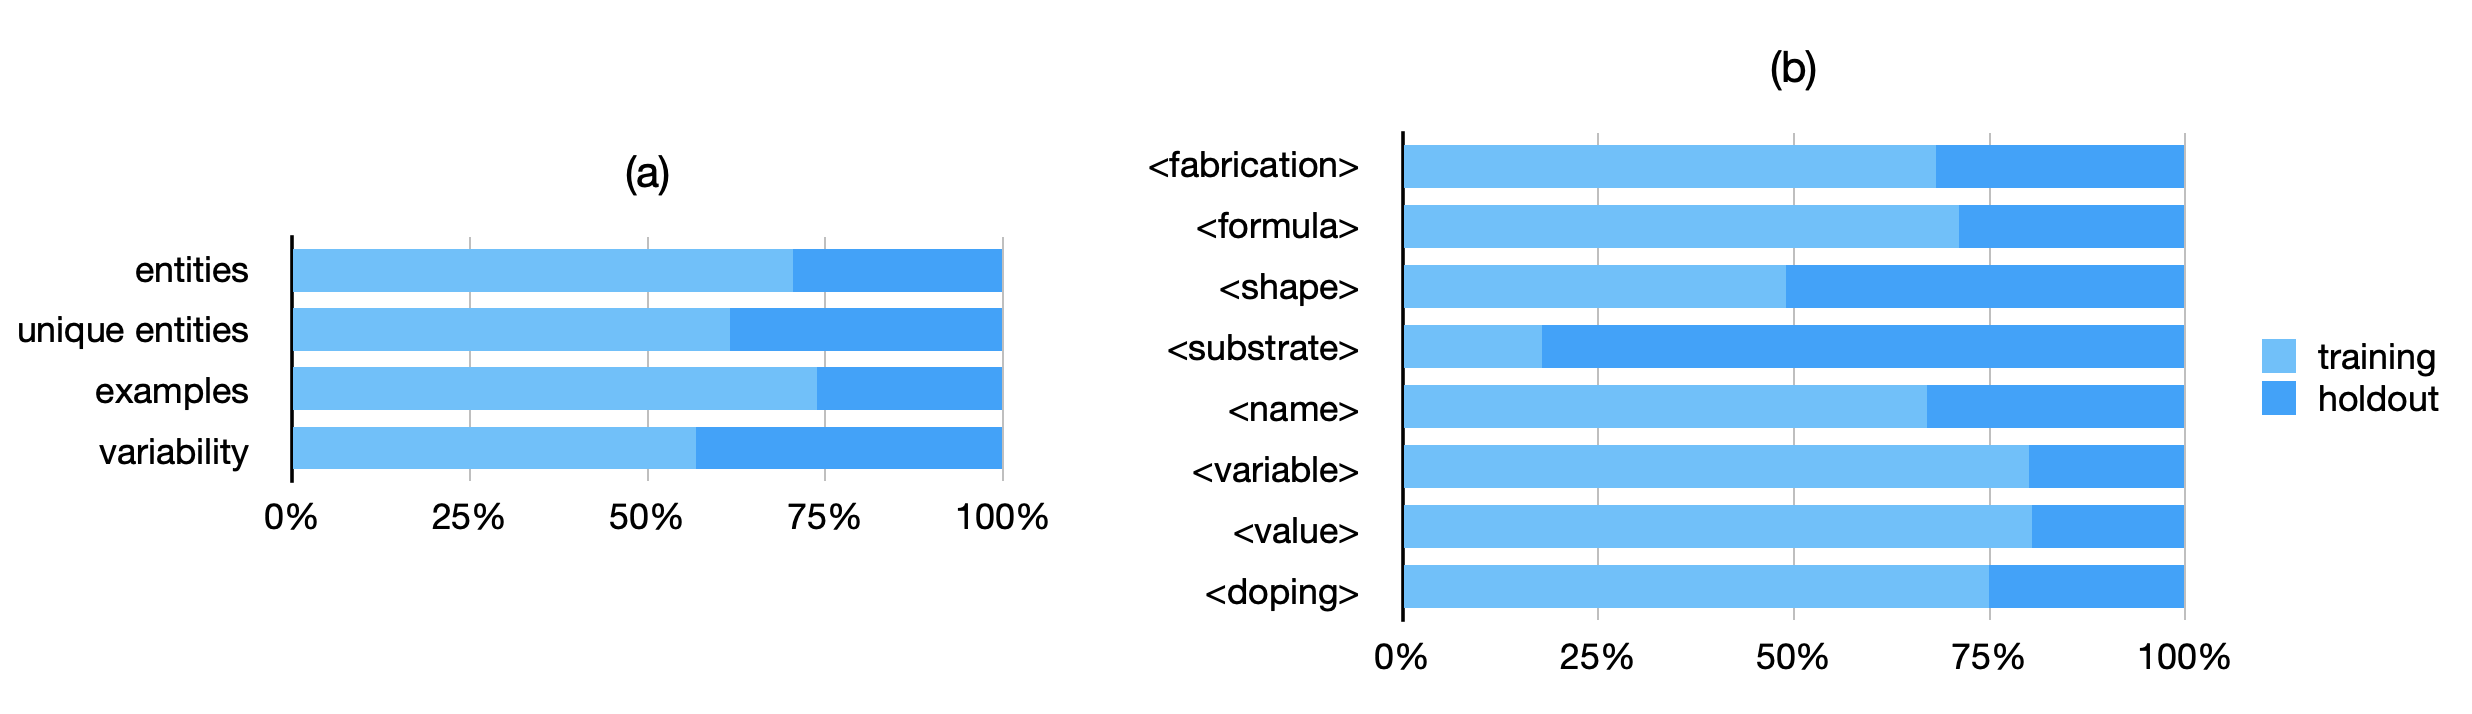
\includegraphics[width=\textwidth]{figures/automatic_extraction_supercon/material-holdout-training-set}
    \caption{Holdout/training set for the Material ML model: (a) general metrics and (b) entity labels.}
    \label{fig:material-training-holdout-set-distribution}
\end{figure}

The resulting holdout set has an average coverage greater than 25\% (Figure~\ref{fig:material-training-holdout-set-distribution}) and an average ``outside the domain'' ratio of 83.93\% (Figure~\ref{fig:material-out-domain-holdout}).

\begin{figure}[ht]
    \centering
    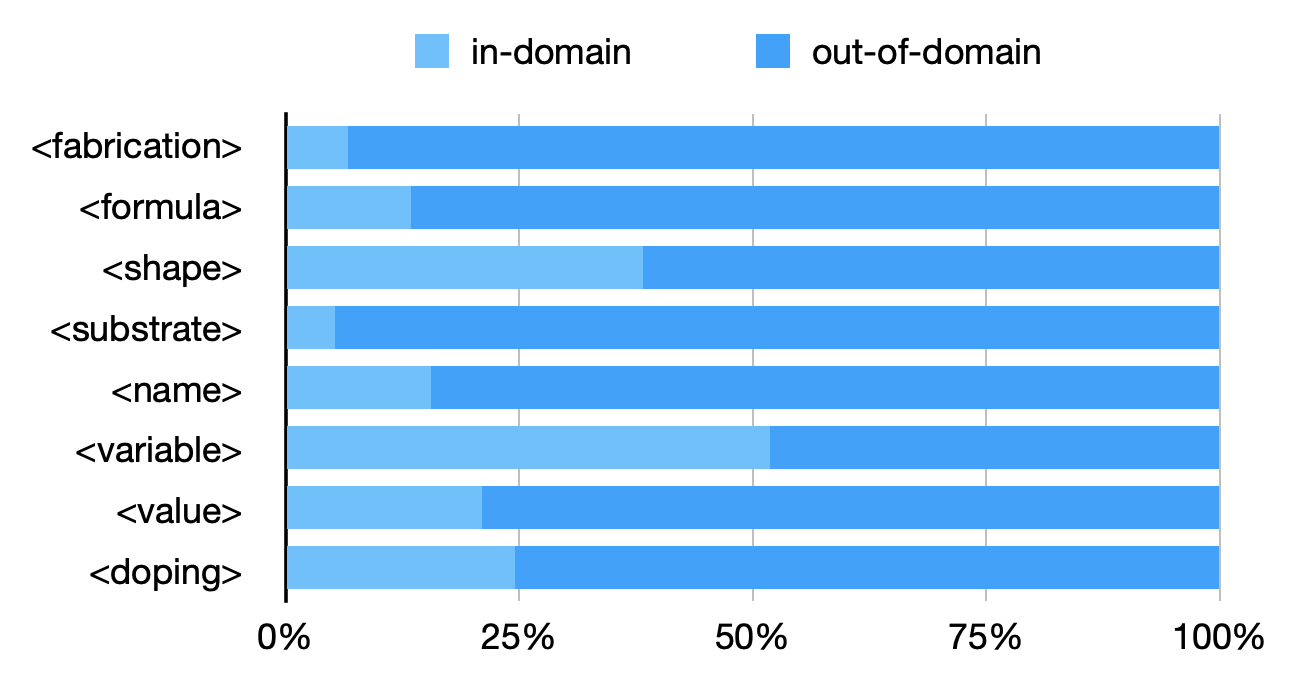
\includegraphics[width=0.6\textwidth]{figures/automatic_extraction_supercon/material-out-domain-holdout-unique}
    \caption{Holdout ``out-of-domain'' rates for the Material ML model. The entities from the holdout set that are also in the training set are the in-domain, and the entities that are not in the training set are the out-of-domain.}
    \label{fig:material-out-domain-holdout}
\end{figure}


\begin{table}[ht]
    \centering
    \caption{Holdout/Training set distribution (\%) between training and holdout sets for the Superconductor ML model. Positive examples indicate the number of sentences with at least one entity, and negative examples the number of sentences with no entities.}
    \begin{tabular}{lccc}
        \toprule
                                      & \textbf{training} & \textbf{holdout} & \textbf{\% holdout/training} \\
        \midrule
        \textbf{documents}         & 132               & 32               & 24.24\%                   \\
        \textbf{examples}          & 16902             & 3905             & 23.10\%                   \\
        \textbf{entities}          & 15586             & 3112             & 19.97\%                   \\
        \textbf{unique entities}   & 6699              & 1372             & 20.48\%                   \\
        \textbf{positive examples} & 8380              & 1776             & 21.19\%                   \\
        \textbf{negative examples} & 8522              & 2129             & 24.98\%                   \\
        \bottomrule
    \end{tabular}
    
    \label{tab:training-holdout-set-distribution-annex}
\end{table}

\begin{table}[ht]
    \centering
    \caption{Holdout/Training set distribution (\%) between training and holdout sets on different labels for the Superconductors ML model.}
    \begin{tabular}{lccc}
        \toprule
        label                 & \textbf{training} & \textbf{holdout} & \textbf{\% holdout/training } \\
        \midrule
        \texttt{<tc>}         & 3741              & 639              & 17.08\%                    \\
        \texttt{<class>}      & 1646              & 271              & 16.46\%                    \\
        \texttt{<material>}   & 6943              & 1649             & 23.75\%                    \\
        \texttt{<me\_method>} & 1883              & 355              & 18.85\%                    \\
        \texttt{<tcValue>}    & 1099              & 157              & 14.29\%                    \\
        \texttt{<pressure>}   & 274               & 41               & 14.96\%                    \\
        \bottomrule
    \end{tabular}
    \label{tab:training-holdout-labels-distribution-annex}
\end{table}

\begin{table}[htbp]
    \centering
    \caption{Holdout/Training set distribution (\%) training and holdout sets for the Material ML model.}
    \begin{tabular}{lccc}
        \toprule
                                    & \textbf{training} & \textbf{holdout} & \textbf{\% holdout/training} \\
        \midrule
        \textbf{examples}        & 13648             & 5728             & 41.97\%                   \\
        \textbf{entities}        & 4512              & 2817             & 62.43\%                   \\
        \textbf{unique entities} & 9268              & 3292             & 35.52\%                   \\
        \bottomrule
    \end{tabular}
    \label{tab:training-holdout-set-material-distribution-annex}
\end{table}

\begin{table}[htbp]
    \centering
    \caption{Holdout/Training set distribution (\%) training and holdout sets on different labels for the Material ML model.}
    \begin{tabular}{lccc}
        \toprule
        label                  & \textbf{training} & \textbf{holdout} & \textbf{\% holdout/training } \\
        \midrule
        \texttt{<fabrication>} & 94                & 44               & 46.81\%                    \\
        \texttt{<formula>}     & 6301              & 2569             & 40.77\%                    \\
        \texttt{<shape>}       & 809               & 841              & 103.96\%                   \\
        \texttt{<substrate>}   & 32                & 148              & 462.50\%                   \\
        \texttt{<name>}        & 1930              & 949              & 49.17\%                    \\
        \texttt{<variable>}    & 1795              & 449              & 25.01\%                    \\
        \texttt{<value>}       & 1895              & 463              & 24.43\%                    \\
        \texttt{<doping>}      & 792               & 265              & 33.46\%                    \\
        \bottomrule
    \end{tabular}
    \label{tab:training-holdout-labels-material-distribution-annex}
\end{table}


\subsubsection{Results}

Scibert obtained the best results, with F1 at 84.15\% (Table~\ref{tab:evaluation-10fold-material-parser}).
Inclusion of features in the BidLSTM\_CRF architecture only improved the results by less than 1\% (from 83.13 to 83.76\%).
The label \texttt{<fabrication>} did not perform well in any architecture, most likely because it is too generic (Table~\ref{tab:material-parser-entities}), and the content is too heterogeneous. Another label, \texttt{<substrate>} has only one-third of the training examples of \texttt{<fabrication>} but obtained results that were three times higher with Scibert, suggesting that \texttt{<fabrication>} should be split into separate and more homogeneous labels.

\begin{sidewaystable}[htbp]
    \centering\small
    \caption{Evaluation scores (\%) of the Material ML model with holdout set. Support (Supp) indicates the number of labels in the training data. Values in bold indicate the highest score. P: precision, R: recall.}

    \scalebox{0.9}{
    \begin{tabular}{l ccc ccc ccc ccc r}
        \toprule
        \textbf{Label}         & \multicolumn{3}{c}{\textbf{CRF}} & \multicolumn{3}{c}{\textbf{BidLSTM\_CRF}} & \multicolumn{3}{c}{\makecell{\textbf{BidLSTM\_CRF}                                                                                                                                                 \\\textbf{\_FEATURES}}} &  \multicolumn{3}{c}{\textbf{SciBERT}} & \textbf{Supp}  \\
        \cmidrule(lr){2-4}\cmidrule(lr){5-7}\cmidrule(lr){8-10}\cmidrule(lr){11-13}\cmidrule(lr){14-14}
                               & \textbf{P}                       & \textbf{R}                                & \textbf{F1}                                        & \textbf{P} & \textbf{R} & \textbf{F1}    & \textbf{P}     & \textbf{R} & \textbf{F1}    & \textbf{P} & \textbf{R}     & \textbf{F1}    &      \\
        \midrule
        \texttt{<doping>}      & 60.41                            & 55.85                                     & 58.04                                              & 67.98      & 62.42      & 64.95          & 69.00          & 62.34      & \textbf{65.43} & 63.58      & 62.79          & 63.16          & 792  \\
        \texttt{<fabrication>} & 40.00                            & 4.55                                      & 8.16                                               & 23.61      & 5.91       & 9.24           & 37.33          & 9.09       & 14.48          & 22.51      & 13.18          & \textbf{16.52} & 94   \\
        \texttt{<formula>}     & 80.81                            & 82.29                                     & 81.54                                              & 82.59      & 84.14      & 83.35          & 83.83          & 85.14      & 84.47          & 84.53      & 86.56          & \textbf{85.53} & 6301 \\
        \texttt{<name>}        & 72.2                             & 63.75                                     & 67.71                                              & 76.29      & 78.76      & 77.43          & 74.51          & 80.38      & 77.33          & 77.18      & 81.86          & \textbf{79.44} & 1930 \\
        \texttt{<shape>}       & 90.89                            & 92.51                                     & 91.69                                              & 90.93      & 95.79      & \textbf{93.29} & 90.33          & 95.74      & 92.96          & 89.67      & 97.20          & 93.28          & 809  \\
        \texttt{<substrate>}   & 37.04                            & 6.76                                      & 11.43                                              & 54.31      & 32.43      & 40.44          & 60.08          & 33.38      & 42.82          & 56.32      & 41.22          & \textbf{47.59} & 32   \\
        \texttt{<value>}       & 80.21                            & 83.15                                     & 81.65                                              & 84.81      & 89.33      & 86.99          & 85.16          & 90.15      & \textbf{87.58} & 83.14      & 85.92          & 84.50          & 1895 \\
        \texttt{<variable>}    & 96.85                            & 95.98                                     & 96.41                                              & 95.19      & 97.77      & 96.46          & 96.32          & 97.90      & \textbf{97.10} & 96.22      & 96.52          & 96.37          & 1795 \\
        \midrule
        All (micro avg)        & 81.15                            & 78.09                                     & 79.59                                              & 82.76      & 83.50      & 83.13          & \textbf{83.20} & 84.33      & 83.76          & 83.11      & \textbf{85.23} & \textbf{84.15} &      \\
        \bottomrule
    \end{tabular}
    }
    
    \label{tab:evaluation-10fold-material-parser}
\end{sidewaystable}

\subsection{RE evaluation}

This rule-based linking was evaluated using the linked entities from SuperMat~\cite{foppiano2021supermat} (Table~\ref{table:evaluation-linking}) and is divided considering each link type.
The F1 score for the \texttt{material-tcValue} was about 80\% with a precision of 88.40\%. 
\texttt{tcValue-pressure} F1 score was 3\% lower than  \texttt{material-tcValue} considering much less data available (support was 118 compared with 726).


\begin{table}[htbp]
    \centering
    \caption{Evaluation scores for the Linking. Support (Supp) indicates the number of labels in the training data. Values in bold indicate the highest score. P: precision, R: recall.}
    \begin{tabular}{lcccc}
        \toprule
        \textbf{Relationship type}          & \textbf{P} & \textbf{R} & \textbf{F1-} & Supp \\
        \midrule
        \textbf{material-tcValue}   & 88.40              & 74.52           & 80.87             & 726     \\
        \textbf{tcValue-pressure}   & 85.71              & 71.52           & 77.98             & 118     \\
        \textbf{me\_method-tcValue} & 62.28              & 65.74           & 63.96             & 151     \\
        \bottomrule
    \end{tabular}

    \label{table:evaluation-linking}
\end{table}



\subsection{End to end evaluation}
\label{sec:end2end}
% What is the end 2 end evaluation? 
End-to-end evaluation (E2EE) measures the capacity of the system from the PDF documents until the final linked results.
We limited the scope of the E2EE to the triplet `material-\tc-pressure' which, at the moment, is the backbone upon which the database is built.
We performed the E2EE on the ``500-papers'' dataset where we manually examined the resulting database as follows: 1) we marked invalid records and 2) we identified the cause of failure from a predefined set of five \textit{error types} (Figure~\ref{fig:error-types}):
\begin{itemize}
    \item \textbf{From table}: the extracted text is wrongly extracted from a table. Although table content is ignored, the error rate from the Grobid library is still relevant due to the lack of training data.
    \item \textbf{Extraction}: entities are not recognised, wrongly recognised, or partially recognised.
    \item \textbf{Quantity extraction}: quantity entities (pressure, temperature) are not correctly extracted. We measured this error separately to identify the failure that could be shared with the Quantity ML model.
    \item \textbf{\tc classification}: the temperature is wrongly classified as superconducting \tc.
    \item \textbf{Linking}: given the initial steps were performed correctly, the resulting entities are not linked correctly.
\end{itemize}

\begin{figure}[htbp]
    \centering
    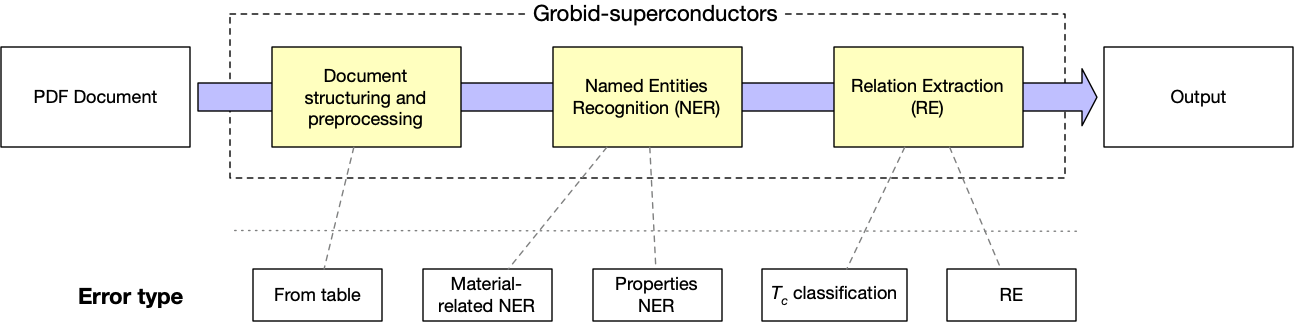
\includegraphics[width=\textwidth]{figures/automatic_extraction_supercon/error-types-colors}
    \caption{\textit{Error types} in the context of the data flow. }
    \label{fig:error-types}
\end{figure}

The E2EE scores are summarised in Table~\ref{table:end2end-evaluation-summary}.
Recall is omitted because it is less relevant and difficult to calculate manually.
The precision score (micro average) was 72.60\% for all the subsections, although the error rates of figure captions (59.28\%) and unknown subsections (57.14\%) were clearly lower than those of the other subsections ($>$ 70\%).
The `unknown` subsections indicate that the extracted text's structure was not well identified by Grobid but it was nevertheless aggregated.
The overall score increases to 73\% when excluding unknown subsections, 75.24\% when excluding figure captions, and 79.14\%  when excluding both.
Excluding these two subsections will not impact the amount of text, because both account for less than 20\% of the total number of subsections.

\begin{figure}[htbp]
    \centering
    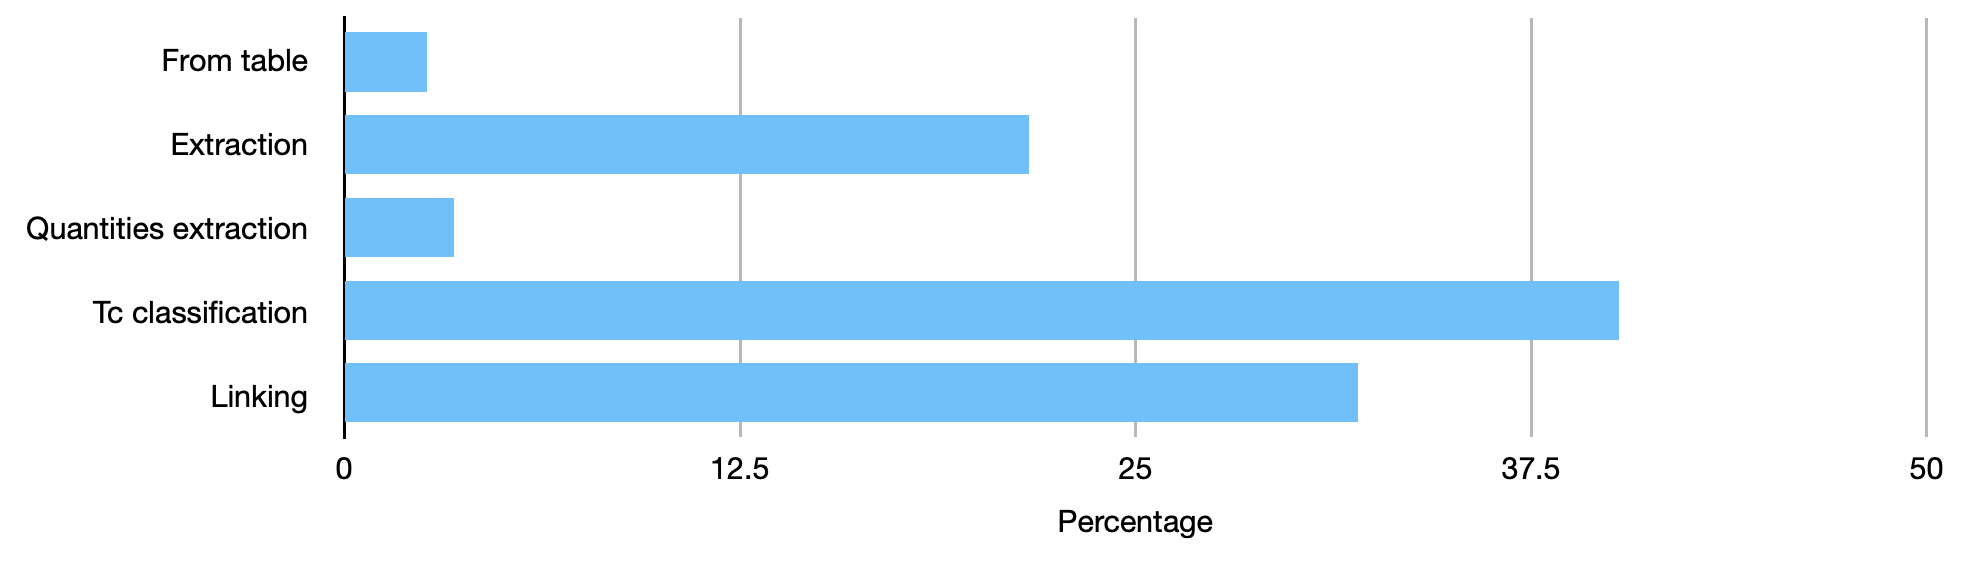
\includegraphics[width=\linewidth]{figures/automatic_extraction_supercon/error-types-bars-perc}
    \caption{Error type distribution in the E2EE of the \textit{500-papers} dataset.}
    \label{fig:error-types-distribution}
\end{figure}

The error types are summarised in Figure~\ref{fig:error-types-distribution}. The most common failures originate from \tc~classification (40\%), Linking (32\%), and Extraction (20\%).
The most common \tc classification failures are as incorrect recognition of 1) relative values of \tc (e.g., 1 K higher than material X); 2) values indicating the transition temperature width ($\Delta T_{c}$); 3) temperature values that are not \tc, for example, material synthesis temperatures ($T$), other critical transition temperatures that are not superconducting (e.g., $T_{Curie}$); and 4) values of temperature at which there is no superconductivity (e.g., ``at 70 K there is no superconductivity'').
``Linking errors'' mainly occur when the text compare relative values of \tc~using materials as the basis for comparison (e.g., ``The Tc = 38 K is similar to the one of MgB$_{2}$'').
Finally, ``Extraction'' issues mainly originate from: 1) implicit mention of the main material when experimented using different ``substrates'' combination, and 2) mismatches between \texttt{<material>} and \texttt{<class>} which, by definition, overlap.


\begin{table}[htbp]
    \centering
    \caption{Summary of the E2EE evaluation scores. Support indicates the number of labels in the training data.}
    \begin{tabular}{l c c}
        \toprule
        \textbf{Subsection}                                      & \textbf{Precision} & \textbf{Support} \\
        \midrule
        Title                                                    & 100                & 2                \\
        Abstract                                                 & 80.32              & 61               \\
        Paragraph                                                & 75.2               & 623              \\
        Figure captions                                          & 59.28              & 140              \\
        Unknown                                                  & 57.14              & 21               \\
        \midrule
        \textbf{Micro avg.}                                      & 72.60              & 847              \\
        \textbf{Micro avg.} (excl. figures)                      & 75.24              & 707              \\
        \textbf{Micro avg.} (excl. unknown sections)             & 73.00              & 603              \\
        \textbf{Micro avg.} (excl. figures and unknown sections) & 79.14              & 657              \\
        \bottomrule
    \end{tabular}
    
    \label{table:end2end-evaluation-summary}
\end{table}

\section{Conclusions}

This work introduces our proposed method for automatically extracting materials and properties. This method is an essential component of our project, which aims to create a database of experimental data sourced from scientific literature.
Our contribution is novel in its use in a previously unexplored area, where the extraction of information is challenging due to the intricate nature of the field and the specific attributes of the entities involved. 

The contribution described in this chapter, has been published in the paper "Automatic extraction of materials and properties from scientific literature"~\cite{foppiano2023automatic} and in "Automatic identification and normalisation of physical quantities from scientific literature"~\cite{foppiano2019quantities}.
